\documentclass[12pt]{article}
\usepackage{amsmath}
\usepackage{tikz}

\begin{document}

\begin{center}
    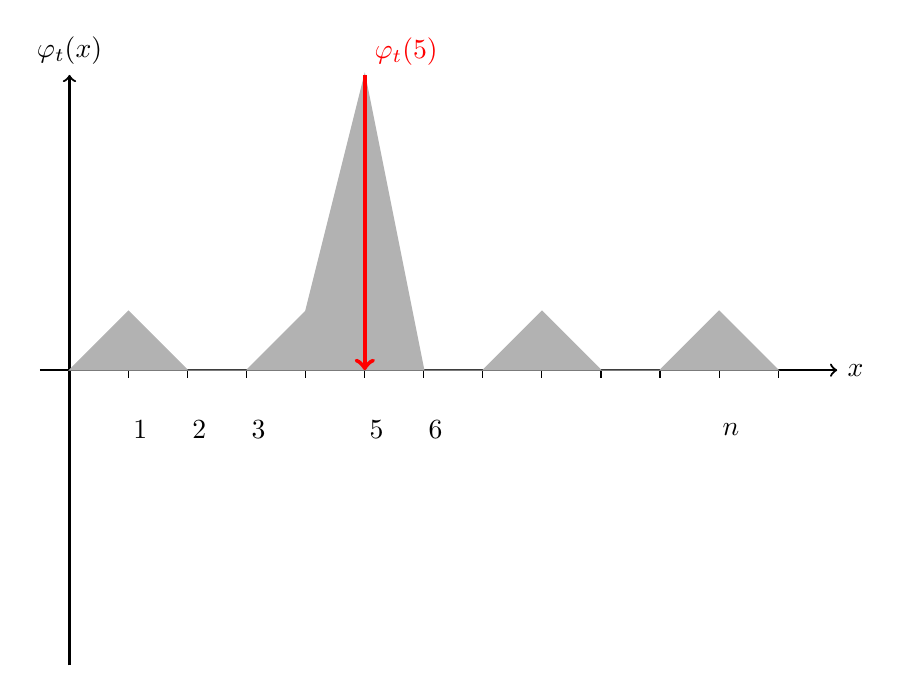
\begin{tikzpicture}[scale=0.75]
        % Axes
        \draw[thick,->] (-0.5,0) -- (13,0) node[right] {$x$};
        \draw[thick,->] (0,-5) -- (0,5) node[above] {$\varphi_t(x)$};

        % Mark points on x-axis
        \foreach \x in {1,...,12}
            {
            \draw (\x,0.2pt) -- ++(0,-4pt);
            }

        % Draw the interface and shaded regions
        \filldraw[gray!60] (0,0) -- (1,1) -- (2,0) -- (3,0) -- (4,1) -- (5,5) -- (6,0) -- (7,0) -- (8,1) -- (9,0) -- (10,0) -- (11,1) -- (12,0) -- cycle;
        \draw[red, ultra thick, ->] (5,5) -- (5,0); % Highlight the position of \varphi_t(5)
        \node[red,above right] at (5,5) {$\varphi_t(5)$};

        % Label the value at 5
        \draw (5.2, -1) node {$5$};

        % Add labels for other points on the x-axis if needed
        \draw (1.2, -1) node {$1$};
        \draw (2.2, -1) node {$2$};
        \draw (3.2, -1) node {$3$};
        \draw (6.2, -1) node {$6$};
        \draw (11.2, -1) node {$n$};
    \end{tikzpicture}
\end{center}

\medskip
The GL dynamics on the lattice $\Lambda_n = \{1,\ldots,n\}$ can be seen as a fluctuating interface conserving the algebraic volume (represented in gray) ${\mathcal V}_n(\varphi_t) := {\mathcal V}_{\Lambda_n}(\varphi_t) = \sum_{x \in \Lambda_n} \varphi_t(x)$ between the interface and the $x$-axis.

\end{document}